%
% slides.tex -- slides
%
% (c) 2017 Prof Dr Andreas Müller, Hochschule Rapperswil
%
\theoremstyle{definition}
\newtheorem{prob}{Problem}
\newtheorem{aufgabe}{Aufgabe}
\newtheorem{loesung}{Lösung}
\newtheorem{idee}{Idee}
\newtheorem{plan}{Plan}
\newtheorem{anomalie}{Übergang zur Anomalie}
\newtheorem{koeffizientenvergleich}{Koeffizientenvergleich}

\begin{document}

\begin{frame}
\frametitle{Grundaufgabe}
Modell in der Form einer Differentialgleichung
\[
\frac{dx}{dt} = f(x,t)
\]
oder ein verallgemeinertes Klimamodell
\[
\frac{d}{dt} Du = Au + N(u)
\]
\begin{prob}
Raum der Lösungsfunktionen $x(t)$ oder $u(t)$ ist unendlichdimensional.
\end{prob}
\begin{aufgabe}
Finde eine Formulierung des Modelles, die nur mit endliche vielen
Parametern auskommt.
\end{aufgabe}
\end{frame}

\begin{frame}
\frametitle{Potenzreihen}
\begin{idee}
Verwende die Funktionen
\[
1, x, x^2, x^2, \dots, x^k,\dots
\]
zur Darstellung der Funktionen:
\[
f(x) = a_0 + a_1 x + a_2 x^2 + a_3 x^3 +\dots
\]
(Taylorreihe)
\end{idee}
\begin{plan}
\begin{itemize}
\item Lösungsansatz $f$ in Problem einsetzen
\item Koeffizientenvergleich: {\color{red}algebraische} Gleichungen für $a_k$
\item Nur endlich viele Koeffizienten berücksitigen $\rightarrow$
endlichdimensionales Modell
\end{itemize}
\end{plan}
\end{frame}

\begin{frame}
\frametitle{Beispiel: $y'=cy$}
\begin{aufgabe}
Finde die Funktion $y(x)$, die die Gleichung
$y'(x) = cy(x)$ erfüllt mit Anfangsbedingung $y(0) = A$
\end{aufgabe}
\begin{loesung}
Lösungsansatz
\[
y(x) = a_0 + a_1x + a_2x^2 + a_3x^3 +a_4x^4+\dots, y(0)=a_0=A
\]
einsetzen:
\[
a_1 + 2a_2x + 3a_3x^2 + \dots = ca_0 + ca_1x + ca_2x^2 + \dots
\]
\end{loesung}
\end{frame}

\begin{frame}

\begin{koeffizientenvergleich}
\vspace{-20pt}
\begin{align*}
&\text{Anfangsbedingung:}     & a_0&=A   &&\Rightarrow& a_0&=A                \\
&\text{Koeffizient von $x^0$:}& a_1&=ca_0&&\Rightarrow& a_1&=Ac               \\
&\text{Koeffizient von $x^1$:}&2a_2&=ca_1&&\Rightarrow& a_2&=A\frac{c^2}{2}   \\
&\text{Koeffizient von $x^2$:}&3a_3&=ca_2&&\Rightarrow& a_3&=A\frac{c^3}{1\cdot 2\cdot 3}\\
&\vdots                       &    &     &&           &    &                  \\
&\text{Koeffizient von $x^k$:}&ka_k&=ca_{k-1}&&\Rightarrow& a_k&=A\frac{c^k}{k!}   \\
\end{align*}
\vspace{-20pt}
\end{koeffizientenvergleich}
Lösung:
$
\displaystyle
y(x)=A\biggl(
\sum_{k=0}^\infty \frac{(cx)^k}{k!}
\biggr)
=
Ae^{cx}.
$
\end{frame}

\begin{frame}
\frametitle{Fourierreihen}
\begin{idee}
Verwende die Funktionen 
\[
1, \cos x, \sin x, \cos 2x, \sin 2x, \dots
\]
zur Darstellung {\color{red}periodischer} Funktionen:
\[
f(x) = \frac{a_0}2 + \sum_{k=1}^\infty (a_k\cos kx + b_k\sin kx)
\]
\end{idee}
\end{frame}

\begin{frame}
\frametitle{Fourierreihen}
\begin{columns}
\begin{column}{0.50\hsize}
\begin{aufgabe}
Löse die Differentialgleichung für die Temperaturverteilung $T(x,t)$
\vspace{-10pt}
\[
\frac{\partial T}{\partial t}
=
\kappa \frac{\partial^2 T}{\partial x^2}
\qquad
t\ge 0, -\pi \le x \le \pi
\]
Mit Randbedingungen
\[
\color{red}
T(-\pi,t) = -T_0,\quad T(\pi,t)=T_0,\quad T(x,0)=0
\]
\vspace{-10pt}
\end{aufgabe}
\end{column}
\begin{column}{0.4\hsize}
\begin{center}
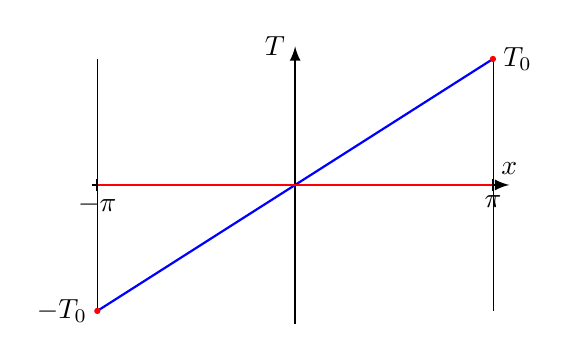
\begin{tikzpicture}[>=latex,thick,scale=0.8]
\draw[->] (-3.23,0)--(3.4,0) coordinate[label=$x$];
\draw[->] (0,-2.2)--(0,2.2) coordinate[label={left:$T$}];
\draw[line width=0.2pt] (-3.14,-2)--(-3.14,2);
\draw[line width=0.2pt] (3.14,-2)--(3.14,2);
\draw (-3.14,-0.1)--(-3.14,0.1);
\draw (+3.14,-0.1)--(+3.14,0.1);
\node at (-3.14,0) [below] {$-\pi$};
\node at (3.14,0) [below] {$\pi$};
\node at (-3.14,-2) [left] {$-T_0$};
\node at (3.14,2) [right] {$T_0$};
\only<2->{
\draw[color=blue] (-3.14,-2)--(3.14,2);
}
\draw[color=red] (-3.13,0)--(3.13,0);
\fill[color=red] (-3.14,-2) circle[radius=0.05];
\fill[color=red] (3.14,2) circle[radius=0.05];
\end{tikzpicture}
\end{center}
\end{column}
\end{columns}
\begin{anomalie}
Abweichung vom linearen Temperaturprofil:
\[
\vartheta(x,t) = T(x,t) - {\color{blue}\frac{T_0}{\pi}x}
\qquad
\Rightarrow
\qquad
\frac{\partial \vartheta}{\partial t} = \frac{\partial T}{\partial t},
\;
\frac{\partial^2\vartheta}{\partial x^2} = \frac{\partial^2 T}{\partial x^2},
\;
\frac{\partial \vartheta}{\partial t}
=
\kappa \frac{\partial^2 \vartheta}{\partial x^2}
\]
\end{anomalie}
\end{frame}

%
%
%
\begin{frame}
\frametitle{Lösung}
Lösungsansatz:
\[
\vartheta(x,t)
=
\frac{a_0(t)}2 + \sum_{k=1}^\infty (a_k(t) \cos kx+b_k(t)\sin kx)
\]
einsetzen:
\begin{align*}
\frac{\partial \vartheta}{\partial t}
&=
\frac{\dot a_0(t)}2
+
\sum_{k=1}^\infty \phantom{k^2}(\dot a_k(t) \cos kx+\dot b_k(t)\sin kx)
\\
\frac{\partial^2\vartheta}{\partial x^2}
&=
\phantom{\frac{\dot a_0(t)}2}
-\sum_{k=1}^\infty k^2(a_k(t) \cos kx+b_k(t)\sin kx)
\end{align*}

\end{frame}

\begin{frame}
\frametitle{Lösung}
Koeffizientenvergleich:
\begin{align*}
\dot a_0(t)&=0                 &&\Rightarrow& a_0(t) = a_0(0)                \\
\dot a_k(t)&=-\kappa k^2 a_k(t)&&\Rightarrow& a_k(t) = a_k(0)e^{-\kappa k^2t}\\
\dot b_k(t)&=-\kappa k^2 b_k(t)&&\Rightarrow& b_k(t) = b_k(0)e^{-\kappa k^2t}
\end{align*}
D.~h.~Problem ist reduziert auf die Bestimmung der $a_k(0)$ und $b_k(0)$
\begin{columns}
\begin{column}{0.5\hsize}
Mit der Fouriertheorie kann man berechnen:
\[
{\color{blue}\vartheta(x,0)}
=
\sum_{k=1}^\infty
\underbrace{
\frac{2(-1)^k}{\pi k}
}_{\displaystyle = b_k(0)} \sin kx
\]
\end{column}
\begin{column}{0.5\hsize}
\begin{center}
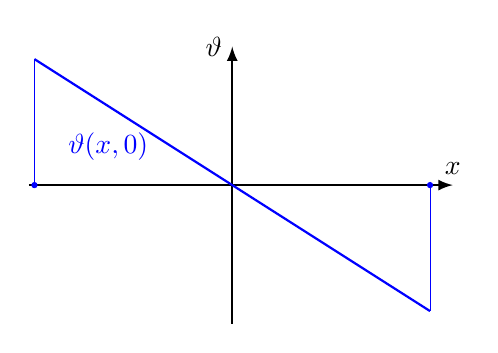
\begin{tikzpicture}[>=latex,thick,scale=0.8]
\draw[->] (-3.23,0)--(3.5,0) coordinate[label=$x$];
\draw[->] (0,-2.2)--(0,2.2) coordinate[label={left:$\vartheta$}];
\draw[color=blue] (-3.14,2)--(3.14,-2);
\fill[color=blue] (-3.14,0) circle[radius=0.05];
\fill[color=blue] (3.14,0) circle[radius=0.05];
\node[color=blue] at ({-1.57+0.4},1) [below left] {$\vartheta(x,0)$};
\draw[color=blue,line width=0.1pt] (-3.14,0)--(-3.14,2);
\draw[color=blue,line width=0.1pt] (3.14,0)--(3.14,-2);
\end{tikzpicture}
\end{center}
\end{column}
\end{columns}
\end{frame}

\def\waermeloesung{
\draw[domain=-180:180,samples=201,color=red]
	plot ({2*3.14159*\x/180},{3*(
	-(2/3.14159)*exp(-\t)*sin(\x)
	+(2/(2*3.14159))*exp(-4*\t)*sin(2*\x)
	-(2/(3*3.14159))*exp(-9*\t)*sin(3*\x)
	+(2/(4*3.14159))*exp(-16*\t)*sin(4*\x)
	-(2/(5*3.14159))*exp(-25*\t)*sin(5*\x)
	+(2/(6*3.14159))*exp(-36*\t)*sin(6*\x)
	-(2/(7*3.14159))*exp(-49*\t)*sin(7*\x)
	+(2/(8*3.14159))*exp(-64*\t)*sin(8*\x)
	-(2/(9*3.14159))*exp(-81*\t)*sin(9*\x)
	+(2/(10*3.14159))*exp(-100*\t)*sin(10*\x)
	-(2/(11*3.14159))*exp(-121*\t)*sin(11*\x)
	+(2/(12*3.14159))*exp(-144*\t)*sin(12*\x)
	-(2/(13*3.14159))*exp(-169*\t)*sin(13*\x)
	+(2/(14*3.14159))*exp(-196*\t)*sin(14*\x)
	-(2/(15*3.14159))*exp(-225*\t)*sin(15*\x)
	+(2/(16*3.14159))*exp(-256*\t)*sin(16*\x)
	)
});
}

\newboolean{waermeanimation}
\setboolean{waermeanimation}{true}
\ifthenelse{\boolean{waermeanimation}}{
\begin{frame}
\frametitle{Vollständige Lösung}
\[
{\color{red}
\vartheta(x,t)
}
=
\sum_{k=1}^\infty \frac{2(-1)^k}{\pi k} e^{-\kappa k^2 t}\sin kx
\]
\begin{center}
\begin{tikzpicture}[>=latex,thick]
\draw[->] (-6.3,0)--(6.5,0) coordinate[label=$x$];
\draw[->] (0,-3)--(0,3) coordinate[label={right:$\vartheta$}];
\ifthenelse{\boolean{presentation}}{}{
\node[color=red] at (1,1.5) [right] {$t=0.01, 0.05, 0.1, 0.2, 0.5, 1, 2, 5, 10$};
}
\only<1>{
\ifthenelse{\boolean{presentation}}{
\node[color=red] at (1,1.5) [right] {$t = 0.01$};
}{}
\def\t{0.01}
\waermeloesung
}
\only<2>{
\ifthenelse{\boolean{presentation}}{
\node[color=red] at (1,1.5) [right] {$t = 0.05$};
}{}
\def\t{0.05}
\waermeloesung
}
\only<3>{
\ifthenelse{\boolean{presentation}}{
\node[color=red] at (1,1.5) [right] {$t = 0.1$};
}{}
\def\t{0.1}
\waermeloesung
}
\only<4>{
\ifthenelse{\boolean{presentation}}{
\node[color=red] at (1,1.5) [right] {$t = 0.2$};
}{}
\def\t{0.2}
\waermeloesung
}
\only<5>{
\ifthenelse{\boolean{presentation}}{
\node[color=red] at (1,1.5) [right] {$t = 0.5$};
}{}
\def\t{0.5}
\waermeloesung
}
\only<6>{
\ifthenelse{\boolean{presentation}}{
\node[color=red] at (1,1.5) [right] {$t = 1$};
}{}
\def\t{1}
\waermeloesung
}
\only<7>{
\ifthenelse{\boolean{presentation}}{
\node[color=red] at (1,1.5) [right] {$t = 2$};
}{}
\def\t{2}
\waermeloesung
}
\only<8>{
\ifthenelse{\boolean{presentation}}{
\node[color=red] at (1,1.5) [right] {$t = 5$};
}{}
\def\t{5}
\waermeloesung
}
\only<9>{
\ifthenelse{\boolean{presentation}}{
\node[color=red] at (1,1.5) [right] {$t = 10$};
}{}
\def\t{10}
\waermeloesung
}
%\draw[domain=-180:180,samples=201,color=red]
%	plot ({2*3.14159*\x/180},{3*(
%	-(2/3.14159)*exp(-\t)*sin(\x)
%	+(2/(2*3.14159))*exp(-4*\t)*sin(2*\x)
%	-(2/(3*3.14159))*exp(-9*\t)*sin(3*\x)
%	+(2/(4*3.14159))*exp(-16*\t)*sin(4*\x)
%	-(2/(5*3.14159))*exp(-25*\t)*sin(5*\x)
%	+(2/(6*3.14159))*exp(-36*\t)*sin(6*\x)
%	-(2/(7*3.14159))*exp(-49*\t)*sin(7*\x)
%	+(2/(8*3.14159))*exp(-64*\t)*sin(8*\x)
%	-(2/(9*3.14159))*exp(-81*\t)*sin(9*\x)
%	+(2/(10*3.14159))*exp(-100*\t)*sin(10*\x)
%	-(2/(11*3.14159))*exp(-121*\t)*sin(11*\x)
%	+(2/(12*3.14159))*exp(-144*\t)*sin(12*\x)
%	-(2/(13*3.14159))*exp(-169*\t)*sin(13*\x)
%	+(2/(14*3.14159))*exp(-196*\t)*sin(14*\x)
%	-(2/(15*3.14159))*exp(-225*\t)*sin(15*\x)
%	+(2/(16*3.14159))*exp(-256*\t)*sin(16*\x)
%	)
%});
\draw[color=blue] (-6.283,3)--(6.283,-3);
\fill[color=blue] (-6.283,0) circle[radius=0.05];
\fill[color=blue] (6.283,0) circle[radius=0.05];
\end{tikzpicture}
\end{center}
\end{frame}
}{}

\begin{frame}
\frametitle{Lorenzsystem}
\begin{columns}
\begin{column}{0.5\hsize}
Strömungsgleichungen:
\begin{align*}
\frac{\partial \Delta \psi}{\partial t}
&=
\nu \Delta^2 \psi + c\frac{\partial \vartheta}{\partial x}
%-\frac{\partial(\psi,\Delta\psi)}{\partial(x,y)}
\\
\frac{\partial \vartheta}{\partial t}
&=
\kappa\Delta \vartheta
+
\frac{T_0}{h_0}\frac{\partial \psi}{\partial x}
%-\frac{\partial(\psi,\vartheta)}{\partial(x,y)}
\end{align*}
\end{column}
\def\t{2.5}
\begin{column}{0.5\hsize}
\begin{center}
\begin{tikzpicture}[>=latex,thick]
\draw[->] (-0.5,0)--(5.5,0) coordinate[label=$x$];
\draw[->] (0,-0.5)--(0,{\t+0.5}) coordinate[label={right:$y$}];
\draw[line width=0.1pt] (5,-0.5)--(5,{\t+0.5});
\draw[line width=0.1pt] (-0.5,\t)--(5.5,\t);
\node at (2.5,0) [below] {$T=0$};
\node at (2.5,\t) [above] {$T=T_0$};
\node at (0,0) [below left] {$0$};
\node at (0,\t) [above left] {$\pi$};
\node at (5,0) [below right] {$\pi/a$};
\end{tikzpicture}
\end{center}
\end{column}
\end{columns}
Lösungsansatz:
\begin{align*}
\psi(x,y)
&=
X(t)
{\color{red}\sin ax \sin y}
\\
\vartheta(x,y)
&=
Y(t)
{\color{red}
\cos ax\sin y
}
+
Z(t)
{\color{red}
\sin 2y
}
\end{align*}
$\Rightarrow$ Reduktion auf drei Variablen $X(t)$, $Y(t)$ und $Z(t)$
\end{frame}

\begin{frame}
\frametitle{Lorenzsystem}
Dreidimensionales DGL-System:
\begin{equation}
\begin{aligned}
\dot X(t)
&=
-\nu(a^2+1)X(t)
+\frac{ac}{a^2+1}Y(t)
\\
\dot Y(t)
&=
\frac{aT_0}{\pi}X(t)
-(a^2+1)\kappa Y(t)
-aX(t)Z(t)
\\
\dot Z(t)
&=
-4\kappa Z(t)
+\frac{a}{2}X(t)Y(t)
\end{aligned}
\notag
\end{equation}
\begin{itemize}
\item
2.~und 3.~Gleichung sind nicht linear.
\item
Lösungen zeigen chaotisches Verhalten.
\end{itemize}
\end{frame}

\end{document}
